\DIFdelbegin \DIFdel{In this section we present results of numerical experiments testing the convergence of TG-NDA and NDA. We first test on a simple one material problem with constant source. The second test consists of two materials and a box source. 
}%DIFDELCMD < 

%DIFDELCMD < %%%
\section{\DIFdel{NDA Accuracy}}
%DIFAUXCMD
\addtocounter{section}{-1}%DIFAUXCMD
%DIFDELCMD < 

%DIFDELCMD < %%%
\DIFdel{To ensure the validity of our results, we first establish that NDA is providing an accurate approximation of the transport equation. We check to see that it sufficiently corrects the diffusion equation, as observed in other studies \mbox{%DIFAUXCMD
\cite{morel-holo, Wang2013}}\hspace{0pt}%DIFAUXCMD
. We ran a number of test problems to observe this behavior. For ease of comparison among the three methods, we display test results in a line-out plot, where $y$ is fixed. We observed the behavior shown to be representative of any line through the domain. Fig. \ref{fig:comparison} illustrates a line-out plot fixed at $y=0.25$, from a one material, one group problem with scattering. NDA shows a significant correction to diffusion, maintaining most of the accuracy of the higher order equation. 
}%DIFDELCMD < \begin{figure}[H]
%DIFDELCMD <     \centering
%DIFDELCMD <     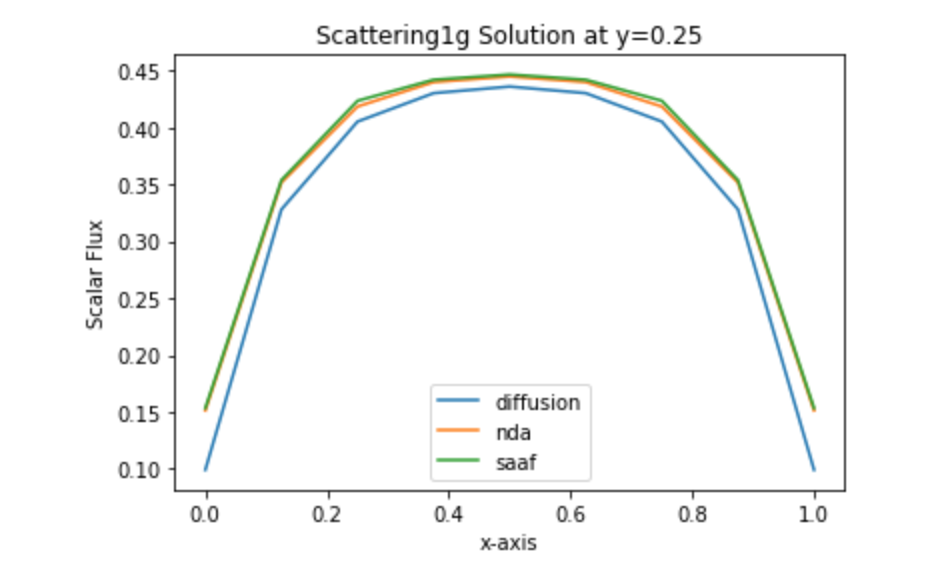
\includegraphics[width=.75\textwidth]{fig/LineOut25.png}
%DIFDELCMD <     %%%
%DIFDELCMD < \caption{%
{%DIFAUXCMD
\DIFdelFL{Comparison of Diffusion, SAAF, and NDA}}
    %DIFAUXCMD
%DIFDELCMD < \label{fig:comparison}
%DIFDELCMD < \end{figure}
%DIFDELCMD < 

%DIFDELCMD < %%%
\DIFdel{We were only able to run the NDA/SAAF comparison for smaller test problems, as the computational cost of running SAAF for our experiments with upscattering was prohibitively high.  However, as the test problems were consistent with the Fig. \ref{fig:comparison}, we assume NDA is faithfully modeling neutron transport. 
}%DIFDELCMD < 

%DIFDELCMD < %%%
\DIFdelend \section{One Material}
%DIF >  Did you tell us how the TG method works in the method section?
%DIF > 
For the first test problem, we used a single material with upscattering throughout a \DIFdelbegin \DIFdel{20cm by 20cm }\DIFdelend \DIFaddbegin \DIFadd{20 by 20
%DIF >  what unit??
 }\DIFaddend domain with a constant \DIFdelbegin \DIFdel{unit sourcethroughout the domain. 
}\DIFdelend \DIFaddbegin \DIFadd{source. 
%DIF >  of what energy? At what location? 
 }\DIFaddend We used cross sections for the seven-group moderator material in the C5G7 benchmark problem\DIFdelbegin \DIFdel{\mbox{%DIFAUXCMD
\cite{C5G7}}\hspace{0pt}%DIFAUXCMD
.  
 }%DIFDELCMD < \begin{table}[!htb]
%DIFDELCMD < \small
%DIFDELCMD < \centering
%DIFDELCMD < %%%
%DIFDELCMD < \caption{%
{%DIFAUXCMD
\DIFdelFL{Scattering Matrix for C5G7 Moderator}}
    %DIFAUXCMD
%DIFDELCMD < \label{tab:two}
%DIFDELCMD < \begin{center}
%DIFDELCMD <     \begin{tabular}{|c|c|c|c|c|c|c|c|}
%DIFDELCMD < \hline
%DIFDELCMD <  & %%%
\DIFdelFL{$\rg'=1$ }%DIFDELCMD < & %%%
\DIFdelFL{2 }%DIFDELCMD < & %%%
\DIFdelFL{3 }%DIFDELCMD < & %%%
\DIFdelFL{4 }%DIFDELCMD < & %%%
\DIFdelFL{5 }%DIFDELCMD < & %%%
\DIFdelFL{6 }%DIFDELCMD < & %%%
\DIFdelFL{7 }%DIFDELCMD < \\ 
%DIFDELCMD < \hline
%DIFDELCMD <  %%%
\DIFdelFL{$1$ }%DIFDELCMD < & %%%
\DIFdelFL{4.44777E-2 }%DIFDELCMD < &  %%%
\DIFdelFL{1.13400E-1 }%DIFDELCMD < & %%%
\DIFdelFL{7.23470E-4 }%DIFDELCMD < & %%%
\DIFdelFL{3.74990E-6 }%DIFDELCMD < & %%%
\DIFdelFL{5.31840E-8     }%DIFDELCMD < &  %%%
\DIFdelFL{0     }%DIFDELCMD < &    %%%
\DIFdelFL{0  }%DIFDELCMD < \\
%DIFDELCMD < \hline
%DIFDELCMD <  %%%
\DIFdelFL{$2$  }%DIFDELCMD < & %%%
\DIFdelFL{0       }%DIFDELCMD < &    %%%
\DIFdelFL{2.82334E-1 }%DIFDELCMD < & %%%
\DIFdelFL{1.29940E-1 }%DIFDELCMD < & %%%
\DIFdelFL{6.23400E-4  }%DIFDELCMD < & %%%
\DIFdelFL{4.80020E-5  }%DIFDELCMD < & %%%
\DIFdelFL{7.44860E-6 }%DIFDELCMD < &  %%%
\DIFdelFL{1.04550E-6 }%DIFDELCMD < \\
%DIFDELCMD < \hline
%DIFDELCMD <  %%%
\DIFdelFL{$3$  }%DIFDELCMD < & %%%
\DIFdelFL{0        }%DIFDELCMD < &      %%%
\DIFdelFL{0  }%DIFDELCMD < &     %%%
\DIFdelFL{3.45256E-1 }%DIFDELCMD < & %%%
\DIFdelFL{2.24570E-1 }%DIFDELCMD < & %%%
\DIFdelFL{1.69990E-2 }%DIFDELCMD < & %%%
\DIFdelFL{2.64430E-3 }%DIFDELCMD < & %%%
\DIFdelFL{5.03440E-4 }%DIFDELCMD < \\
%DIFDELCMD < \hline
%DIFDELCMD <  %%%
\DIFdelFL{$4$  }%DIFDELCMD < & %%%
\DIFdelFL{0          }%DIFDELCMD < &     %%%
\DIFdelFL{0    }%DIFDELCMD < &       %%%
\DIFdelFL{0     }%DIFDELCMD < &  %%%
\DIFdelFL{9.10284E-2 }%DIFDELCMD < & %%%
\DIFdelFL{4.15510E-1 }%DIFDELCMD < & %%%
\DIFdelFL{6.37320E-2 }%DIFDELCMD < & %%%
\DIFdelFL{1.21390E-2 }%DIFDELCMD < \\
%DIFDELCMD < \hline
%DIFDELCMD <  %%%
\DIFdelFL{$5$  }%DIFDELCMD < & %%%
\DIFdelFL{0        }%DIFDELCMD < &       %%%
\DIFdelFL{0     }%DIFDELCMD < &      %%%
\DIFdelFL{0     }%DIFDELCMD < & %%%
\DIFdelFL{7.14370E-5 }%DIFDELCMD < & %%%
\DIFdelFL{1.39138E-1 }%DIFDELCMD < & %%%
\DIFdelFL{5.11820E-1 }%DIFDELCMD < & %%%
\DIFdelFL{6.12290E-2 }%DIFDELCMD < \\
%DIFDELCMD < \hline
%DIFDELCMD < %%%
\DIFdelFL{$6$  }%DIFDELCMD < & %%%
\DIFdelFL{0        }%DIFDELCMD < &       %%%
\DIFdelFL{0   }%DIFDELCMD < &    %%%
\DIFdelFL{0      }%DIFDELCMD < &  %%%
\DIFdelFL{0     }%DIFDELCMD < &  %%%
\DIFdelFL{2.21570E-3 }%DIFDELCMD < & %%%
\DIFdelFL{6.99913E-1 }%DIFDELCMD < &  %%%
\DIFdelFL{5.37320E-1 }%DIFDELCMD < \\
%DIFDELCMD < \hline
%DIFDELCMD < %%%
\DIFdelFL{$7$  }%DIFDELCMD < & %%%
\DIFdelFL{0       }%DIFDELCMD < &        %%%
\DIFdelFL{0        }%DIFDELCMD < &   %%%
\DIFdelFL{0      }%DIFDELCMD < &     %%%
\DIFdelFL{0      }%DIFDELCMD < &     %%%
\DIFdelFL{0   }%DIFDELCMD < &    %%%
\DIFdelFL{1.32440E-1 }%DIFDELCMD < & %%%
\DIFdelFL{2.48070E+0 }%DIFDELCMD < \\
%DIFDELCMD < \hline
%DIFDELCMD <     \end{tabular}
%DIFDELCMD < \end{center}
%DIFDELCMD < \end{table}
%DIFDELCMD < 

%DIFDELCMD < %%%
\DIFdelend \DIFaddbegin \DIFadd{. \mbox{%DIFAUXCMD
\cite{C5G7}}\hspace{0pt}%DIFAUXCMD
.  
}\DIFaddend The problems were run on a single \DIFdelbegin \DIFdel{2.7 GHz Intel Core i5 }\DIFdelend processor of a MacBook Pro and the results are show in Table~\ref{tab:onemat}.
%DIF >  what are the details of the processor?
\begin{table}[!htb]
\centering
\caption{Runtime and GS Iteration Count for One Material Problem}
    \label{tab:onemat}
\begin{center}
    \begin{tabular}{|c|c|c|}
    \hline
    & Runtime (s) & GS Iterations \\
    \hline
    \DIFdelbeginFL %DIFDELCMD < 

%DIFDELCMD <     %%%
\DIFdelendFL TG-NDA & 5,465 & 9 \\
    NDA & 14,513 & 31 \\
    \hline
    \end{tabular}
\end{center}
\end{table}
\DIFdelbegin %DIFDELCMD < 

%DIFDELCMD < %%%
\DIFdelend %DIF >  match # of sigfigs... also, I just cut the fractions of seconds as they seemed unimportant  and added commas for readability. Could also covert to sci notation.
The two-grid method provides a considerable acceleration of the Gauss Seidel method. \DIFdelbegin \DIFdel{It is able to converge in roughly 30\% the number of iterations and roughly 37\% the time. }\DIFdelend While when using TG-NDA each iteration takes slightly longer as the correction term must be calculated, there is a considerable decrease in the number of iterations necessary to reach convergence. 
%DIF >  may want to add average time / iteration to table to facilitate the comparison

Importantly, the acceleration in convergence came at no cost to accuracy. As can be seen in Figure~\ref{fig:Moderator}, the NDA and TG-NDA solutions have the same values (up to tolerance). In the interest of space, we only show the results from the highest energy group, but the agreement between NDA and TG-NDA held for all energy groups in our test problems. 
\DIFdelbegin \DIFdel{The full results can be found on github at www.github.com/mzweig/gallo/test/benchmarks.
}%DIFDELCMD < 

%DIFDELCMD < %%%
\DIFdelend %DIF >  and the full set of data can be found at location...
\begin{figure}[H]
\centering
\begin{subfigure}{.5\textwidth}
  \centering
  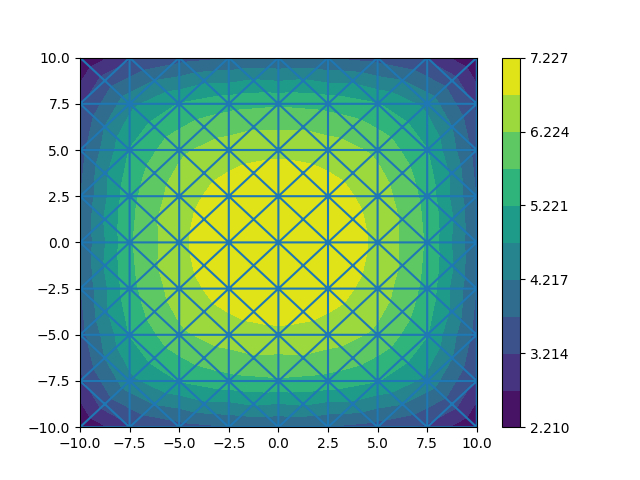
\includegraphics[width=\linewidth]{fig/nda_c5g7mod_scalar_flux_group0.png}
  \caption{Highest Energy Group, NDA Scalar Flux}
  \label{fig:NDA-Mod}
\end{subfigure}%
\begin{subfigure}{.5\textwidth}
  \centering
  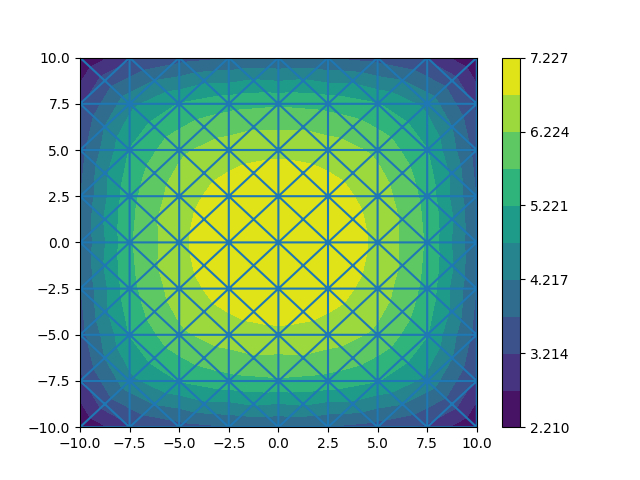
\includegraphics[width=\linewidth]{fig/tgnda_c5g7mod_scalar_flux_group0.png}
  \caption{Highest Energy Group, TG-NDA Scalar Flux}
  \label{fig:TG-NDA-Mod}
\end{subfigure}
\caption{Comparison of NDA and TG-NDA in Scalar Flux for the One Material Problem}
\label{fig:Moderator}
\end{figure}
% please add units

\section{Two Materials}
The second problem consists of two materials in a concentric, box geometry, shown in Figure ~\ref{fig:test_geometry}. 
The first material, located in the center and outer layer, is the C5G7 moderator material used above and the second material has the same total cross sections and pattern of upscattering, but with higher absorption and lower total scattering. Both materials have seven groups. 
\DIFdelbegin %DIFDELCMD < 

%DIFDELCMD <  \begin{table}[!htb]
%DIFDELCMD < \small
%DIFDELCMD < \centering
%DIFDELCMD < %%%
%DIFDELCMD < \caption{%
{%DIFAUXCMD
\DIFdelFL{Scattering Matrix for Second Material}}
    %DIFAUXCMD
%DIFDELCMD < \label{tab:two}
%DIFDELCMD < \begin{center}
%DIFDELCMD <     \begin{tabular}{|c|c|c|c|c|c|c|c|}
%DIFDELCMD < \hline
%DIFDELCMD <  & %%%
\DIFdelFL{$\rg'=1$ }%DIFDELCMD < & %%%
\DIFdelFL{2 }%DIFDELCMD < & %%%
\DIFdelFL{3 }%DIFDELCMD < & %%%
\DIFdelFL{4 }%DIFDELCMD < & %%%
\DIFdelFL{5 }%DIFDELCMD < & %%%
\DIFdelFL{6 }%DIFDELCMD < & %%%
\DIFdelFL{7 }%DIFDELCMD < \\ 
%DIFDELCMD < \hline
%DIFDELCMD < %%%
\DIFdelFL{1 }%DIFDELCMD < & %%%
\DIFdelFL{4.387665E-2 }%DIFDELCMD < & %%%
\DIFdelFL{1.13400E-1   }%DIFDELCMD < &  %%%
\DIFdelFL{7.23470E-4 }%DIFDELCMD < & %%%
\DIFdelFL{3.74990E-6 }%DIFDELCMD < & %%%
\DIFdelFL{5.31840E-8  }%DIFDELCMD < &     %%%
\DIFdelFL{0    }%DIFDELCMD < &     %%%
\DIFdelFL{0    }%DIFDELCMD < \\
%DIFDELCMD < \hline
%DIFDELCMD < %%%
\DIFdelFL{2 }%DIFDELCMD < & %%%
\DIFdelFL{0        }%DIFDELCMD < &    %%%
\DIFdelFL{2.8231821E-1  }%DIFDELCMD < & %%%
\DIFdelFL{1.29940E-1 }%DIFDELCMD < & %%%
\DIFdelFL{6.23400E-4 }%DIFDELCMD < & %%%
\DIFdelFL{4.80020E-5 }%DIFDELCMD < & %%%
\DIFdelFL{7.44860E-6 }%DIFDELCMD < & %%%
\DIFdelFL{1.04550E-6 }%DIFDELCMD < \\
%DIFDELCMD < \hline
%DIFDELCMD < %%%
\DIFdelFL{3 }%DIFDELCMD < & %%%
\DIFdelFL{0       }%DIFDELCMD < &        %%%
\DIFdelFL{0    }%DIFDELCMD < &       %%%
\DIFdelFL{3.44919E-1 }%DIFDELCMD < & %%%
\DIFdelFL{2.24570E-1 }%DIFDELCMD < & %%%
\DIFdelFL{1.69990E-2 }%DIFDELCMD < & %%%
\DIFdelFL{2.64430E-3 }%DIFDELCMD < & %%%
\DIFdelFL{5.03440E-4 }%DIFDELCMD < \\
%DIFDELCMD < \hline
%DIFDELCMD < %%%
\DIFdelFL{4 }%DIFDELCMD < & %%%
\DIFdelFL{0         }%DIFDELCMD < &      %%%
\DIFdelFL{0      }%DIFDELCMD < &         %%%
\DIFdelFL{0     }%DIFDELCMD < &  %%%
\DIFdelFL{8.90878E-2 }%DIFDELCMD < & %%%
\DIFdelFL{4.15510E-1 }%DIFDELCMD < & %%%
\DIFdelFL{6.37320E-2 }%DIFDELCMD < & %%%
\DIFdelFL{1.21390E-2 }%DIFDELCMD < \\
%DIFDELCMD < \hline
%DIFDELCMD < %%%
\DIFdelFL{5 }%DIFDELCMD < & %%%
\DIFdelFL{0     }%DIFDELCMD < &          %%%
\DIFdelFL{0       }%DIFDELCMD < &        %%%
\DIFdelFL{0   }%DIFDELCMD < &    %%%
\DIFdelFL{7.14370E-5 }%DIFDELCMD < & %%%
\DIFdelFL{1.33396E-1 }%DIFDELCMD < & %%%
\DIFdelFL{5.11820E-1 }%DIFDELCMD < & %%%
\DIFdelFL{6.12290E-2 }%DIFDELCMD < \\
%DIFDELCMD < \hline
%DIFDELCMD < %%%
\DIFdelFL{6 }%DIFDELCMD < & %%%
\DIFdelFL{0   }%DIFDELCMD < &        %%%
\DIFdelFL{0      }%DIFDELCMD < &         %%%
\DIFdelFL{0   }%DIFDELCMD < &        %%%
\DIFdelFL{0     }%DIFDELCMD < &  %%%
\DIFdelFL{2.21570E-3 }%DIFDELCMD < & %%%
\DIFdelFL{6.84912E-1 }%DIFDELCMD < & %%%
\DIFdelFL{5.37320E-1 }%DIFDELCMD < \\
%DIFDELCMD < \hline
%DIFDELCMD < %%%
\DIFdelFL{7 }%DIFDELCMD < & %%%
\DIFdelFL{0      }%DIFDELCMD < &         %%%
\DIFdelFL{0        }%DIFDELCMD < &       %%%
\DIFdelFL{0    }%DIFDELCMD < &       %%%
\DIFdelFL{0    }%DIFDELCMD < &       %%%
\DIFdelFL{0    }%DIFDELCMD < &   %%%
\DIFdelFL{1.32440E-1 }%DIFDELCMD < & %%%
\DIFdelFL{2.443461  }%DIFDELCMD < \\
%DIFDELCMD < \hline
%DIFDELCMD <     \end{tabular}
%DIFDELCMD < \end{center}
%DIFDELCMD < \end{table}
%DIFDELCMD < 

%DIFDELCMD < %%%
\DIFdelend %DIF >  can you include a table of the cross section values used? At least for the scattering? It would help us see the structure since this depends a lot on the scattering structure.  
There is a box source in the center that emits 70\% in the highest energy group, 20\% in the second-highest, and 10\% in the third-highest energy group.
\begin{figure}[H]
    \centering
    
\includegraphics[width=.3\textwidth]{fig/Geometry.png}
    \caption{Geometry of Two-Material Test Problem}
    \label{fig:test_geometry}
\end{figure}

\begin{table}[!htb]
\centering
\caption{Runtime and GS Iteration Count for Two Material Problem}
    \label{tab:two}
\begin{center}
    \begin{tabular}{|c|c|c|}
    \hline
    & Runtime (s) & GS Iterations \\
    \hline
    TG-NDA & 4,222 & 8 \\
    NDA & 10,382 & 25 \\
    \hline
    \end{tabular}
\end{center}
\end{table}

The test results are in Table ~\ref{tab:two}. Again, TG-NDA showed a significant improvement over the unaccelerated Gauss Seidel, taking roughly \DIFdelbegin \DIFdel{taking roughly 40\% of the time and 32\% of the iterations }\DIFdelend \DIFaddbegin \DIFadd{one third the number of iterations as NDA alone}\DIFaddend . Again, NDA and TG-NDA agree in terms of flux values. Figure~\ref{fig:Moderator2} also \DIFaddbegin \DIFadd{only }\DIFaddend shows results for the highest energy group 
\DIFdelbegin \DIFdel{and one of the thermal groups. The full results can be found on github at www.github.com/mzweig/gallo/test/benchmarks.
}%DIFDELCMD < 

%DIFDELCMD < %%%
\DIFdelend %DIF >  and again, the full set of data can be found... 
\begin{figure}[H]
\centering
\begin{subfigure}{.5\textwidth}
  \centering
  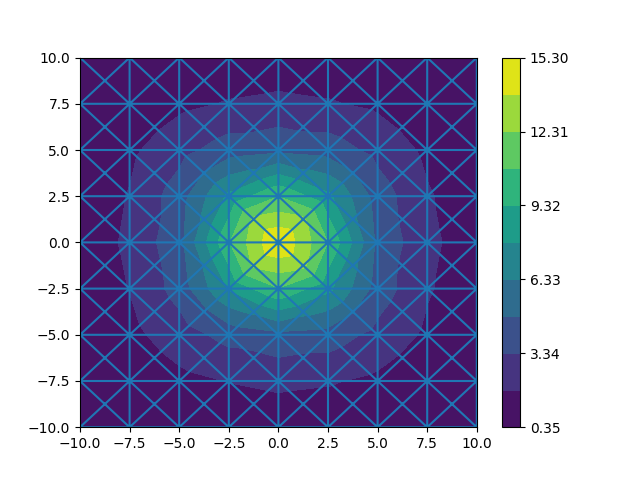
\includegraphics[width=\linewidth]{fig/nda_iron-water_scalar_flux_group0.png}
  \caption{Highest Energy Group, NDA}
  \label{fig:NDA-Mod2}
\end{subfigure}%
\begin{subfigure}{.5\textwidth}
  \centering
  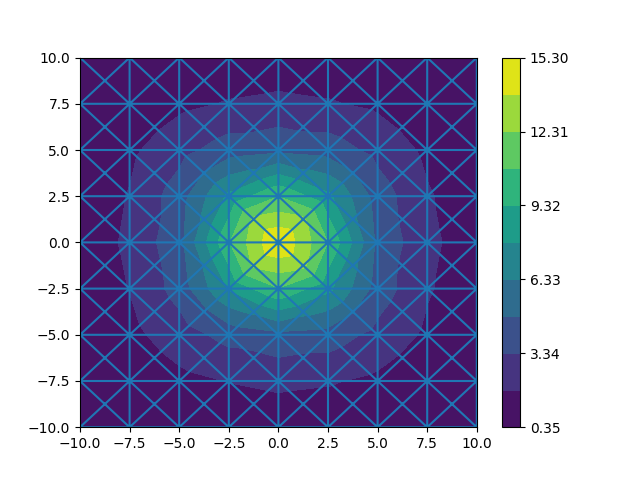
\includegraphics[width=\linewidth]{fig/tgnda_iron-water_scalar_flux_group0.png}
  \caption{Highest Energy Group, TG-NDA}
  \label{fig:TG-NDA-Mod2}
\end{subfigure}
\caption{Comparison of NDA and TG-NDA in Scalar Flux for the Two Material Problem}
\label{fig:Moderator2}
\DIFdelbeginFL %DIFDELCMD < \end{figure}
%DIFDELCMD < 

%DIFDELCMD < \begin{figure}[H]
%DIFDELCMD < \centering
%DIFDELCMD < \begin{subfigure}{.5\textwidth}
%DIFDELCMD <   \centering
%DIFDELCMD <   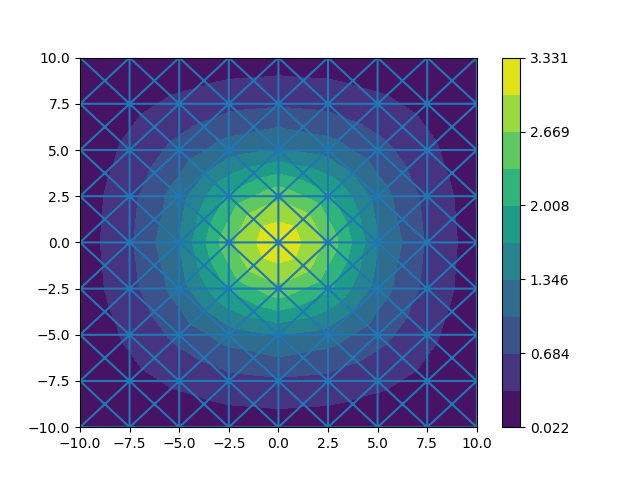
\includegraphics[width=\linewidth]{fig/nda_iron-water_scalar_flux_group3.png}
%DIFDELCMD <   %%%
%DIFDELCMD < \caption{%
{%DIFAUXCMD
\DIFdelFL{First Thermal Energy Group, NDA}}
  %DIFAUXCMD
%DIFDELCMD < \label{fig:NDA-Mod}
%DIFDELCMD < \end{subfigure}%%%
%DIF < 
%DIFDELCMD < \begin{subfigure}{.5\textwidth}
%DIFDELCMD <   \centering
%DIFDELCMD <   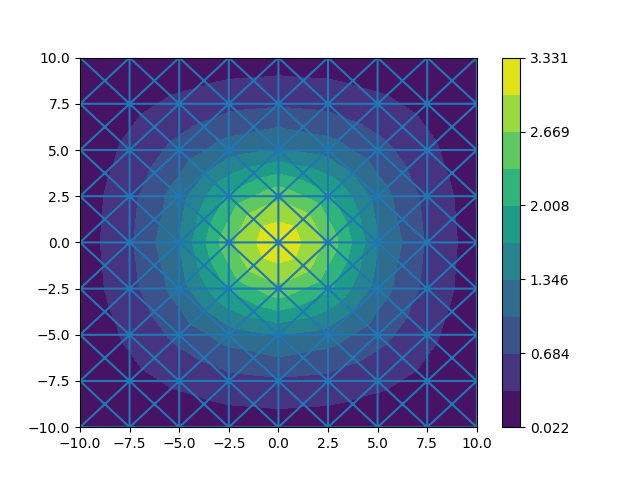
\includegraphics[width=\linewidth]{fig/tgnda_iron-water_scalar_flux_group3.png}
%DIFDELCMD <   %%%
%DIFDELCMD < \caption{%
{%DIFAUXCMD
\DIFdelFL{First Thermal Energy Group, TG-NDA}}
  %DIFAUXCMD
%DIFDELCMD < \label{fig:TG-NDA-Mod}
%DIFDELCMD < \end{subfigure}
%DIFDELCMD < %%%
%DIFDELCMD < \caption{%
{%DIFAUXCMD
\DIFdelFL{Comparison of NDA/TG-NDA in Flux Value for Two Material Problem}}
%DIFAUXCMD
%DIFDELCMD < \label{fig:Moderator}
%DIFDELCMD < %%%
\DIFdelendFL \end{figure}

\section{Reproducibility}
The code used to run these experiments is hosted online at www.github.com/mzweig/gallo. The version used is tagged as masters-thesis. The geometry inputs \texttt{origin-centered10} and material input \texttt{c5g7mod} were used for the first test problem, and the geometry input \texttt{iron-water10} and material input \texttt{mod-water} were used for the second problem. 